\chapter*{capitulo 7 ejercicio 7}
\textbf{a) Estblesca una suma de integrales definidade que represente el área sombreada total entre las curvas $y=f(x)$ e $y=g(x)$ en la siguiente figura. b)Encuentra el área total encerrada entre $y=x^3$ e $y=x$ en el intervalo $[-1, 2]$.}
\begin{figure*}[!hbt]
	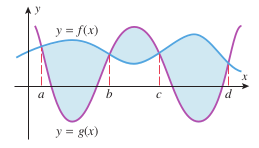
\includegraphics[height = 0.20\textheight]{recursos/image.png}\par
\end{figure*}

Si \( f \) y \( g \) son funciones continuas en el intervalo \([a, b]\), y si \( f(x) \geq g(x) \) para todo \( x \) en \([a, b]\), entonces el área de la región delimitada por \( y = f(x) \) arriba, \( y = g(x) \) abajo, a la izquierda por la línea \( x = a \), y a la derecha por la línea \( x = b \) es \[ A = \int_{a}^{b} [f(x) - g(x)] \, dx \]

Entonces se puede observar que $f(x)\geq g(x)$ en el intervalo $[a,b]$ $\therefore$ el área de la región dada  $f(x)$ y $ g(x)$ es $$A_1=\int_{a}^{b}\bigg[f(x)-g(x)\bigg]dx$$

Por otro lado se puede observar que $f(x)\leq g(x)$ $\forall x\in[b,c]$ $\therefore$ el área está dada como $$A_2=\int_{b}^{c}\bigg[g(x)-f(x)\bigg]dx$$

Del mismo modo, el análisis de la región acotada por el intervalo $[c,d]$, observamos que $f(x)\geq g(x)$ $\forall x\in[c,d]$ $\therefore$ el área se describe como $$A_3=\int_{c}^{d}\bigg[f(x)-g(x)\bigg]dx$$
Entonces el área total etá dada por la suma de estas tres áreas indiciduales tal que
$$A_T=\int_{a}^{b}\bigg[f(x)-g(x)\bigg]dx + \int_{b}^{c}\bigg[g(x)-f(x)\bigg]dx + \int_{c}^{d}\bigg[f(x)-g(x)\bigg]dx$$

De este modo tenemos en cuenta los casos cuando $f(x)\geq g(x)$ y $f(x)\leq g(x)$
\\
b)Encuentra el área total encerrada entre $y=x^3$ e $y=x$ en el intervalo $[-1, 2]$.
Sean $y=f(x)=x$ y $y=g(x)=x^3$
¿Cuándo pasa que son iguales?
\begin{align*}
	f(x)=g(x)\iff x_1 & =x_2^3       \\
	f(x)=g(x)\iff 0   & =x_2^3-x     \\
	f(x)=g(x)\iff 0   & =x(x-1)(x+1) \\
\end{align*}
Son iguales en $x=0$, $x=1$ y $x=-1$

\newpage Procedemos a hacee el análisis de desigualdedes
\begin{table}[!hbt]
	\begin{center}
		\begin{tabular}{| c | c | c | c | c |}
			\hline
			\multicolumn{5}{ |c| }{Análisis de los intervalos}                 \\ \hline
			intervalo   & Punto de prueba & $f(x)$      & $g(x)$ & desigualdad \\ \hline
			($-1,0]$    & -1/2            & $-1/2     $ & $-1/8$ & $f<g$       \\
			($0,1\big]$ & 1/2             & $     1/2$  & $1/8$  & $f>g$       \\
			($1,2\big]$ & 3/2             & $3/2    $   & $27/8$ & $f<g$       \\\hline
		\end{tabular}
		\caption{tabla de análsis de signos de las regiones }
		\label{tab: tabla de análsis de signos de las regiones }
	\end{center}
\end{table}

Entonces aplicando la definición anterior, el area total está dada por
\begin{align*}
	A_T & =\int_{-1}^{0}[g(x)-f(x)]dx+\int_{0}^{1}[f(x)-g(x)]dx+ \int_{1}^{2}[g(x)-f(x)]dx                                 \\
	A_T & =\int_{-1}^{0}[x^3-x)]dx+\int_{0}^{1}[x-x^3]dx+ \int_{1}^{2}[x^3-x]dx                                            \\
	A_T & =\int_{-1}^{0}x^3dx-\int_{-1}^{0}xdx+\int_{0}^{1}xdx-\int_{0}^{1}x^3dx+ \int_{1}^{2}x^3dx-\int_{1}^{2}xdx        \\
	A_T & =\bigg(\frac{x^4}{4}-\frac{x^2}{2}\bigg)\bigg|^0_{-1}+\bigg(\frac{x^2}{2}-\frac{x^4}{4}\bigg)\bigg|_0^1+ \bigg(\frac{x^4}{4}-\frac{x^2}{2}\bigg)\bigg|_1^2 \\
	A_T & =-\bigg(\frac{-1^4}{4}-\frac{-1^2}{2}\bigg)+\bigg(\frac{1^2}{2}-\frac{1^4}{4}\bigg)+ \bigg(\frac{2^4}{4}-\frac{2^2}{2}\bigg)-\bigg(\frac{1^4}{4}-\frac{1^2}{2}\bigg) \\
	A_T & =\frac{1}{4}+\frac{1}{4}+ \bigg(4-2\bigg)+\frac{1}{4} \\
	A_T & =\frac{1}{2}+ 2+\frac{1}{4} \\
	A_T & =0.5+ 2 +0.25\\
	A_T & =2.75\\
\end{align*}

el área total es 2.75 unidades de área